\chapter{NeedFinding}
\href{https://drive.google.com/drive/u/0/folders/1XoItlFMNVkWT7CER1GdP-kYDjVKPnojq}{Link alla cartella sul NeedFinding}.

Nell'ambito del nostro progetto, il needfinding è stato applicato per esplorare e comprendere le necessità legate alle infrastrutture verdi. Questo processo ha coinvolto interviste e questionari digitali per raccogliere feedback da parte di diversi gruppi di utenti, con l'obiettivo di identificare le problematiche comuni, le aspettative e le aree di miglioramento nelle attuali soluzioni verdi.
Il needfinding lo abbiamo suddiviso in due macro fasi:
\begin{itemize}
    \item Interviste di persona agli utenti
    \item Questionari digitali sottoposti ad oltre 100 persone
\end{itemize}
abbiamo svolto un totale di 20 interviste, di cui alcune direttamente nei luoghi interessati ( parchi, ville, ecc…) ed un totale di 119 risposte ottenute dai questionari.
Qui di seguito vengono riportate le domande e un riassunto di ciò che è emerso dalle interviste e dai questionari.
\section{Domande delle interviste}
\begin{enumerate}
    \item Quanti anni hai?

    Motivazione: domanda introduttiva per capire la fascia di età dell'intervistato.
    \item A quante infrastrutture verdi riesci ad arrivare a piedi da casa tua?
    
    Motivazione: domanda introduttiva per capire di quante infrastrutture verdi è a conoscenza l'intervistato.
    \item Sei a conoscenza di iniziative o eventi nelle infrastrutture verdi della tua città? Se si quali? Qual'è l'ultima a cui hai partecipato?
    
    Motivazione: domanda introduttiva per sapere se è informato sugli eventi e cosa fa per informarsi.
    \item L'ultima volta che hai usato una nuova infrastruttura verde, come l'hai cercata? Hai mai avuto problemi nella ricerca?

    Motivazione: domanda per capire eventuali need e problemi nel processo di ricerca di un'infrastruttura verde.
\end{enumerate}
L'ultima volta che hai frequentato un'infrastruttura verde (potrebbe essere anche in quel momento):
\begin{enumerate}\setcounter{enumi}{4}
    \item Come hai raggiunto il luogo? Perchè?

    Motivazione: conoscere il modo utilizzato dall'utente per raggiungere il luogo e quali sono le motivazioni.
    \item Hai avuto difficoltà nel trovare o accedere all'infrastruttura? Se sì, quali sono state le principali cause?
    
    Motivazione: conoscere delle possibili problematiche che l'utente può aver riscontrato nell'accedere a questi luoghi, ad esempio se erano chiusi e non lo sapevo, ecc...
    \item Perché l'hai scelta?

    Motivazione: conoscere cosa ha portato l'utente a fare quella scelta e perché rispetto ad altri luoghi.
    \item E' un luogo che consente queste attività: attrezzature sportive, relax, picnic, servizi igienici, aree di ristorazione, aree per cani?

    Motivazione: conoscere eventuali mancanze nell'infrastruttura o nella conoscenza del luogo da parte dell'utente
    \item In una scala da 1 a 5, come valuti la tua esperienza? Perché (cosa intendi con N)?

    Motivazione: conoscere la valutazione personale dell'utente sulla sua esperienza e capirne il motivo.
    \item Hai utilizzato infrastrutture verdi diverse o preferisci sempre questa? Perché?
    
    Motivazione: conoscere cosa ha portato l'utente a fare quella scelta e perché rispetto ad altri luoghi.
    \item Quali sono le 3 caratteristiche essenziali che un'infrastruttura verde deve avere per te?
    
    Motivazione: conoscere le necessità degli utenti in un'infrastruttura verde
    \item Hai mai incontrato persone con interessi simili ai tuoi in queste infrastrutture? Se sì, come interagisci con loro?
    
    Motivazione: conoscere le necessità degli utenti riguardo alle interazioni sociali e agli interessi comuni nelle infrastrutture verdi.
\end{enumerate}
Le risposte raccolte evidenziano che, pur essendo molto apprezzati, i parchi urbani e le ville presentano diverse problematiche che ne limitano l'utilizzo. Uno dei problemi principali riguarda l'accessibilità: spesso i parchi sono difficili da raggiungere, poco segnalati e alle volte non hanno informazioni al loro interno che fanno intendere dove e se ci sono determinati servizi, rendendo complicato il loro utilizzo per alcune persone. C'è anche una carenza evidente di servizi essenziali, come bagni, aree attrezzate per picnic, punti di ristoro, reti Wi-fi pubbliche, e molti lamentano una manutenzione insufficiente, soprattutto in riferimento alla pulizia del parco.
Un altro aspetto critico è la scarsa comunicazione e la poca conoscenza di attività da parte degli utenti; infatti le attività e gli eventi organizzati all'interno dei parchi sono poco pubblicizzati e conosciuti, e questo limita la partecipazione e l'uso del parco come luogo di aggregazione sociale.

\section{Domande del questionario}
\begin{enumerate}
    \item Quanti anni hai?
	
    Motivazione: domanda introduttiva per conoscere la fascia di età.
    \item Qual'è il tuo genere? ( Uomo, Donna, Altro: )

    Motivazione: domanda introduttiva per conoscereil sesso.
    \item Qual è la tua attuale occupazione? ( Lavoratore, Studente, Altro:)
    
    Motivazione: domanda introduttiva per conoscere l'occupazione della persona
\end{enumerate}

Domande sulle infrastrutture verdi
\begin{enumerate}\setcounter{enumi}{3}
    \item Conosci iniziative o eventi nelle infrastrutture verdi che frequenti? ( Per niente, Poco, Abbastanza, Molto)

    Motivazione: Comprendere quanto è a conoscenza l'utente su eventi e iniziative.

    \item Seleziona per ogni domanda la risposta che più si avvicina al tuo caso.
    
    \begin{figure}[ht]
        \centering
        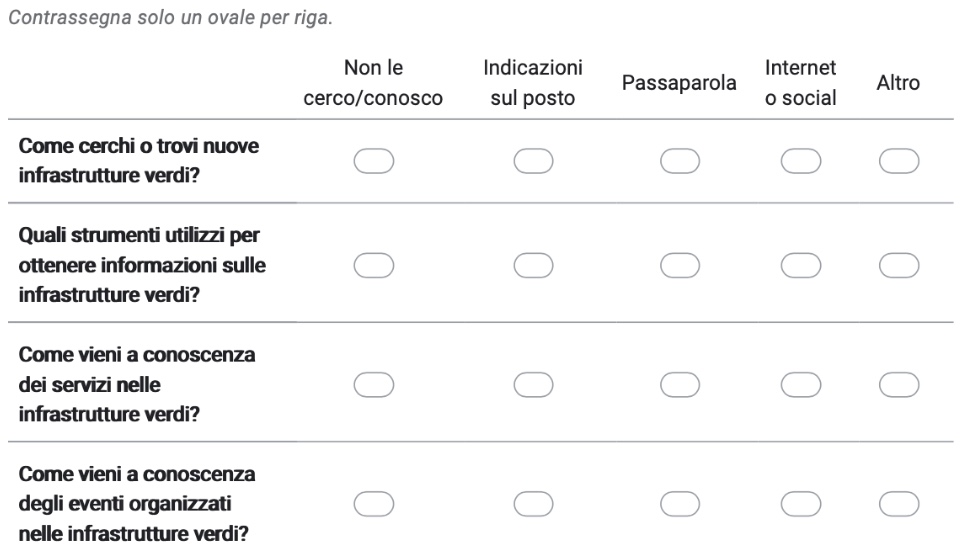
\includegraphics[width=0.7\linewidth]{images/domanda-questionario-5.jpg}
    \end{figure}
    Motivazione: Venire a conoscenza delle modalità di come l'utente ottiene nuove informazioni ( se le ottiene) su infrastrutture verdi, i loro eventi, le loro informazioni ed i servizi al loro interno.

    \item Quali problemi hai trovato nelle infrastrutture verdi che hai frequentato? 
    \begin{itemize}
        \item Difficoltà di accesso 
        \item Scarsa manutenzione 
        \item Poca sicurezza 
        \item Troppo affollamento
        \item Pochi servizi
        \item Altro: ...
    \end{itemize}
    Motivazione: Venire a conoscenza dei possibili problemi che l'utente ha riscontrato frequentando le infrastrutture verdi, lasciando spazio a risposte multiple ed una risposta aperta 
    \item Come valuti l'accessibilità delle infrastrutture verdi che hai frequentato? ( Da 1 a 4, 1=Pessima, 4=Eccellente)
    
    Motivazione: Conoscere il grado di valutazione dell'utente sull'accessibilità delle infrastrutture verdi che ha frequentato; domanda posta per indagare di più sul problema venuto fuori dalle interviste
    \item Come valuti la pulizia delle infrastrutture verdi che hai frequentato? ( Da 1 a 4, 1=Pessima, 4=Eccellente)
    
    Motivazione: Comprendere quanto l'utente reputa pulite le infrastrutture che ha frequentato
    \item Quando è stata l'ultima volta che hai frequentato un'infrastruttura verde?
    \begin{itemize}
        \item 1/2 giorni fa
        \item Nell'ultima settimana
        \item Nell'ultimo mese
        \item Più di un mese fa
    \end{itemize}

    Motivazione: Venire a conoscenza dell'ultima volta che l'utente ha frequentato un'infrastruttura verde
    \item L'ultima volta che hai frequentato un'infrastruttura verde come l'hai raggiunta?
    \begin{itemize}
        \item A piedi
        \item Mezzi pubblici
        \item Bicicletta
        \item Auto/moto
        \item Altro…
    \end{itemize}

    Motivazione: Venire a conoscenza del modo in cui l'utente raggiunge le infrastrutture verdi

    \item L'ultima volta che hai frequentato un'infrastruttura verde, aveva a disposizione questi servizi?

    \begin{figure}[ht]
        \centering
        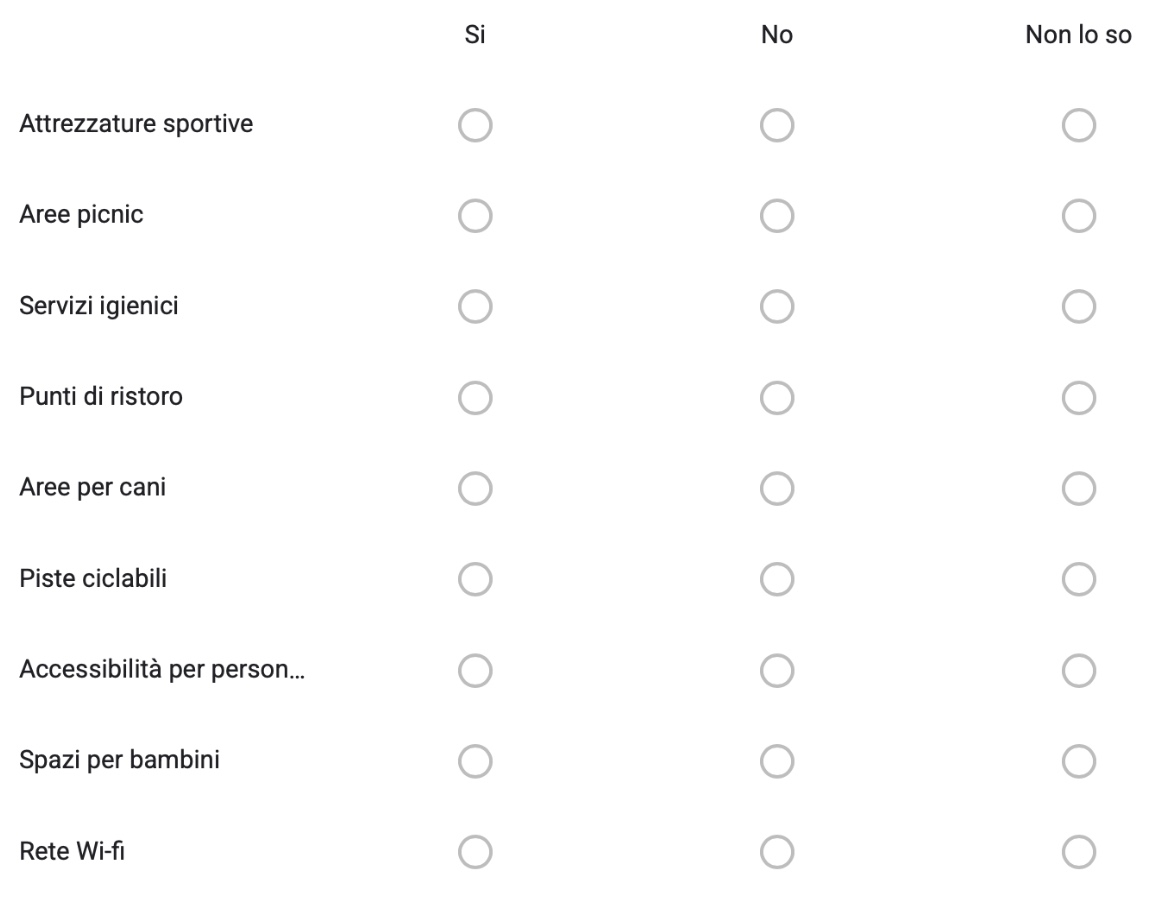
\includegraphics[width=0.7\linewidth]{images/domanda-questionario-11.jpg}
    \end{figure}
    
    Motivazione: Comprendere la conoscenza dell'utente sulla presenza o meno di determinati servizi 
 
    \item Come preferisci svolgere le tue attività nelle infrastrutture verdi?
    \begin{itemize}
        \item Da solo 
        \item In compagnia
    \end{itemize}
    Motivazione: Comprendere se l'utente preferisce svolgere attività in compagnia o da solo, per poi indagare se ha problemi nel trovare persone con le quali svolgere le attività
    \item Riesci a trovare persone con interessi simili nelle infrastrutture verdi? (da 1 a 4, 1 = Difficilmente, 4 = Facilmente)
	
    Motivazione: Scoprire se l'utente ha problemi nel trovare persone con interessi simili ai propri

    \item Riesci ad interagire con persone con interessi simili nelle infrastrutture verdi? (da 1 a 4, 1 =Poco, 4 = Molto)
    
    Motivazione: Scoprire se l'utente ha problemi nell'interagire con persone con interessi simili ai propri

    \item Quali suggerimenti hai per migliorare l'esperienza complessiva nelle   infrastrutture verdi?
    
    Motivazione: Ricevere feed dall'utente e scoprire informazioni e suggerimenti non trattati nel questionario per scovare ancora più need.

    \item Ci sono altri problemi legati alle infrastrutture verdi che non abbiamo affrontato e che vorresti segnalarci?
    
    Motivazione: Ricevere feed dall'utente e scoprire informazioni e suggerimenti non trattati nel questionario per scovare ancora più need.
\end{enumerate}